\subsection{Merkle Trees}
Consider a set $S = \{s_1, s_2, \cdots, s_n\}$ of strings
$s_i \in \{0, 1\}^*$. At some initial time, this set is compressed into a
\emph{root} string $s$ which is short ($|s| = \lambda$). This compressed string
is produced honestly and is given to a party called the \emph{verifier}. Given
this short trusted root string, the verifier receives claims from untrusted
\emph{provers} which claim that a certain piece of data $e$ existed in $S$.
The verifier's job is to decide whether such claims are truthful or fraudulent.

This protocol is an \emph{authenticated set}\index{Authenticated Set}. It consists of
four algorithms $\mathcal{G}$, $\textsc{compress}$, $\textsc{prove}$,
$\textsc{verify}$. At the beginning of the execution, $\mathcal{G}(1^\lambda)$
is invoked to initialize the protocol parameters. These parameters can be shared
among multiple invocations of the protocol. As these parameters are fixed by the
protocol in its concrete implementations, we will make them implicit from now
on. A set $S$ is compressed by invoking $\textsc{compress}(S)$
which produces the root $s$. When an honest prover wishes to prove that some
element $e$ exists in $S$, they produce an \emph{inclusion proof}\index{Inclusion Proof} $\pi =
\textsc{prove}(S, e)$. When the verifier receives an element $e$ together
with an inclusion proof $\pi$, they check its veracity by invoking
$\textsc{verify}(\pi, e, s)$, which returns $\true$ or $\false$.

Authenticated set protocols must be correct. This means that honest
executions should always work.

\begin{definition}[Correctness]
  Consider an authenticated set protocol
  $\Pi = (\textsc{compress},\allowbreak \textsc{prove},\allowbreak \textsc{verify})$.
  We say that $\Pi$ is
  \emph{correct} if

  \[\forall S:
    \forall e \in S:
    \textsc{verify}(\textsc{prove}(S, e), e, \textsc{compress}(S))\,.\]
\end{definition}

Such protocols are useful when $s$ and $\pi$ are short.

\begin{definition}[Succinctness]
  Consider an authenticated set protocol
  $\Pi = (\textsc{compress},\allowbreak \textsc{prove},\allowbreak \textsc{verify})$.
  We say that $\Pi$ is
  \emph{succinct} if
  for all $S$ it holds that

  \[|\textsc{compress}(S)| \in \bigO(polylog(|S|))
    \land
    \forall e \in S:
    |\textsc{prove}(S, e)| \in \bigO(polylog(|S|))
    \,.\]
\end{definition}

In the protocols we will explore, we will have $|s| = \lambda \in \bigO(1)$ and
$\pi \in \bigO(\log(|S|))$. Furthermore, $|S|$ will be polynomial in $\lambda$.

An authenticated set protocol is \emph{secure} if no adversary can
convince a verifier about the inclusion of an element which is not in the
set. This is made formal in the game illustrated in
Algorithm~\ref{alg.authenticated}.

\begin{figure}[t]
\begin{algorithm}[H]
    \caption{\label{alg.authenticated} The authenticated data structure challenger.}
    \begin{algorithmic}[1]
        \Function{\sf AUTH$_{\Pi,\mathcal{A}}$}{$\lambda$}
            \Let{(S, s_i, \pi)}{\mathcal{A}(1^\lambda)}
            \State\Return{$s_i \not\in S \land \textsc{verify}(\textsc{compress}(S), s_i, \pi)$}
        \EndFunction
        \vskip8pt
    \end{algorithmic}
\end{algorithm}
\end{figure}


\begin{definition}[Security]
  An authenticated set protocol $\Pi = (\textsc{compress},\allowbreak \textsc{prove},\allowbreak \textsc{verify})$ is \emph{secure} if for all PPT adversaries $\mathcal{A}$
  there is a negligible function $\negl$ such that

  \[
    \Pr[\textsf{AUTH}_{\Pi,\mathcal{A}}(\lambda)] < negl(\lambda)\,.
  \]
\end{definition}

A construction that solves this problem which is used extensively in blockchain
protocols is the \emph{Merkle Tree}~\cite{merkle}\index{Merkle Tree}. This construction is
illustrated in Algorithm~\ref{alg.merkle}. It is parameterized by a hash
function $H$. The construction presented works for $|S|$ equal to a power of
$2$.

It treats $S$ as a sequence and organizes it into a complete binary tree $Z$
using the $\textsf{heapify}$ routine. The routine places the hashes of the
elements of $S$ on the leaves of $Z$ by storing them at locations $Z[|S|{:}]$.
The value of each internal node is the hash of the concatenation of the values
of its children. The $\textsf{compress}$ function returns the value of the root
which resides at $Z[1]$. To create a proof $\pi$, the $\textsf{prove}$ routine
takes an index of an element $i$ and finds its position in the binary tree,
namely the leaf stored at $Z[|S| + i]$. It then traverses the path from that
leaf up to the root, maintaining the index of the current node in the variable
$i$. In every iteration, it includes a bit indicating whether the current node
is a left child ($b = 0$) or a right child ($b = 1$). For each node, it includes
the value $Z[i \xor 1]$ of the node's sibling, which has index $i \xor 1$. To
verify a proof, the verifier successively hashes the element whose inclusion is
proven with the hashes $h$ of the siblings provided in the proof $\pi$ on the
correct side indicated by $b$. In the end, it checks whether it has arrived at
the trusted root $s$ and this determines the result of the verification.

Correctness is achieved because the hash function is deterministic and
\textsc{verify} applies hashes in the same manner as \textsc{heapify} does.
Succinctness follows because $|s| = \lambda$ and, furthermore, the tree contains
$2|S| - 1$ elements so the height of the tree is $\Theta(\log(|S|))$, making
$|\pi| \in \Theta(\log(|S|))$.

The construction prefixes the value of each tree node with an indicator string
marking it as a hash (``h:''). On the contrary, each of the elements of $S$ is
marked as content by prefixing it with a different indicator (``c:'') prior to
compressing. The verifier then begins by marking the claimed value as content by
prefixing it with a ``c:'', in which case it can be certain there will be no
confusion with a hash. This ensures that the adversary cannot claim inclusion of
internal nodes as leafs.

\begin{remark}[Length of a Merkle Tree]
  Instead of marking every node as a \emph{hash} or \emph{content} node, the
  \textsf{compress} function can also be made to return the count $|S|$ in
  addition to $s$. In that case, the verifier first asserts that
  $|\pi| = \log|S|$ before proceeding with verification. The compressed string
  has length $\Theta(\log\log|S|)$, but each proof is smaller by a constant
  factor. While this simplifies the security proof, most blockchain protocols
  require that $|s| \in \Theta(1)$ and so we adopt this formulation here.
\end{remark}

Security follows by a direct computational reduction from the collision
resistance of $H$. As this proof is folklore and does not appear in the
literature\footnote{The proof that appears in Modern
Cryptography~\cite{katz} shows something weaker: that a Merkle Tree is a
collision resistant hash function.}, we include our own version here.

\begin{algorithm}[H]
    \caption{\label{alg.merkle} The Merkle Tree construction for $|S| = 2^k$ for
                                some $k$.}
    \begin{algorithmic}[1]
        \Function{\sf heapify$^H$}{$S$}
            \Let{Z[|S|{:}]}{\textsf{map}(H, S)}
            \For{$i \gets |S| - 1 \text{ down to } 1$}
                \Let{Z[i]}{H(Z[2i] \concat Z[2i + 1])}
            \EndFor
            \State\Return{$Z$}
        \EndFunction
        \Function{\sf compress$^H$}{$S$}
            \State\Return{$\textsf{heapify}^H(S)$[1]}
        \EndFunction
        \Function{\sf prove$^H$}{$S, i$}
            \Let{Z}{\textsf{heapify}^H(S)}
            \Let{i}{|S| + i}
            \Let{\pi}{[\,]}
            \While{$i > 1$}
                \Let{b}{i \mod 2}
                \Let{\pi}{\pi \concat (b, Z[i \xor 1])}
                \Let{i}{\lfloor i / 2\rfloor}
            \EndWhile
            \State\Return$\pi$
        \EndFunction
        \Function{\sf verify$^H$}{$\pi, s_i, s$}
            \Let{s_i}{H(s_i)}
            \For{$(b, h) \in \pi$}
                \If{$b$}
                    \Let{s_i}{H(s_i \concat h)}
                \Else
                    \Let{s_i}{H(h \concat s_i)}
                \EndIf
            \EndFor
            \State\Return{$s_i = s$}
        \EndFunction
        \vskip8pt
    \end{algorithmic}
\end{algorithm}


\begin{theorem}[Security]
  Let $H$ be a collision resistant hash function. The Merkle Tree
  construction of Algorithm~\ref{alg.merkle} parameterized by $H$ is a secure
  authenticated set protocol for sets of size $|S| = 2^k$.
\end{theorem}
\begin{proof}
Consider an arbitrary adversary $\mathcal{A}$ against \textsf{AUTH}. We
construct a collision resistance adversary $\mathcal{A}^*$ for the hash function
$H$. The adversary $\mathcal{A}^*$ invokes $\mathcal{A}$ and obtains a proof
$\pi$, an element $e$ and a set $S$. The adversary $\mathcal{A}^*$ checks that
this proof is fraudulent by ensuring that it passes $\textsf{verify}$ and that
$e \not\in S$ (if not, then $\mathcal{A}^*$ aborts). This proof implicitly
encodes a position $i$ in the tree, namely the position expressed by the binary
number obtained by concatenating all the bits $b$ in $\pi$.

First consider the case $|\pi| = \log|S|$. The adversary $\mathcal{A}^*$
checks whether $H(e) = H(S_i)$. If so, it returns the pair $(e, S_i)$ as a
collision. Otherwise it proceeds to find a collision as follows.

\begin{figure}[tb]%{{{
  \centering
  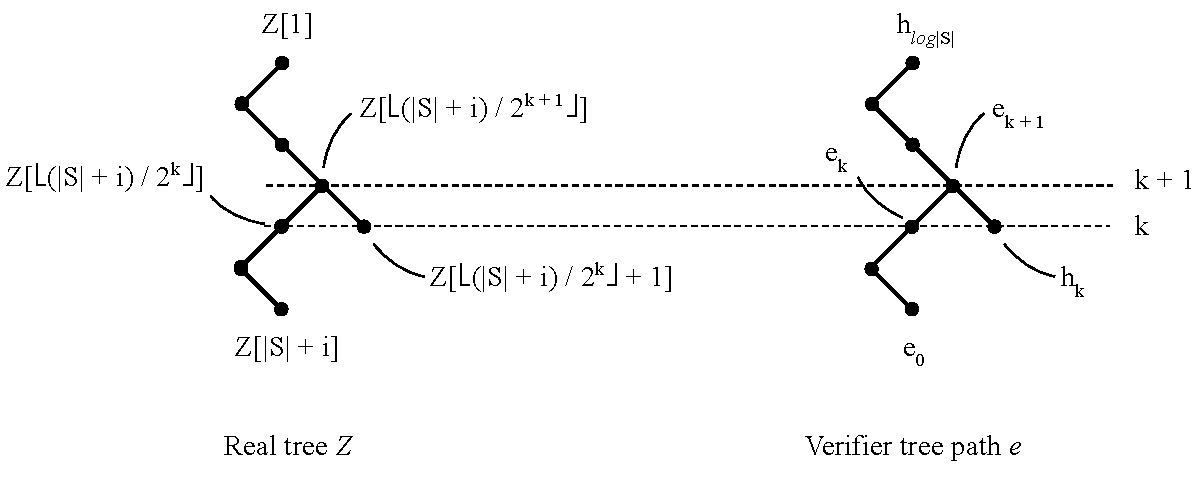
\includegraphics[width=\textwidth]{chapters/background/figures/mtpf.pdf}
  \caption{
    The path comparison between the real tree (left) $Z$ constructed using
    \textsf{heapify} and the verifier tree path (right) $h$ constructed by
    taking successive hashes with the sequence $s_i$ finds a collision at level
    $k$.
  }
  \label{fig.mtpf}
\end{figure}%}}}

The verifier who applies successive hashing will arrive at a
sequence of hashes $e_0, e_1, \cdots, e_{\log|S|}$. The
adversary $\mathcal{A}^*$ evaluates this sequence in the same manner as the
verifier would and also looks at the values $Z[|S| + i], Z[\lfloor \frac{|S| + 1}{2} \rfloor],
\cdots, Z[1]$ as obtained by $\textsc{heapify}(S)$. The adversary
$\mathcal{A}^*$ compares the two sequences and finds the minimum $k \geq 0$ such that
$Z[\lfloor \frac{|S| + i}{2^k} \rfloor] \neq e_k$, but
$Z[\lfloor \frac{|S| + i}{2^{k + 1}} \rfloor] = e_{k + 1}$. This is illustrated
in Figure~\ref{fig.mtpf}.
If $b_k = 0$,
then it returns the pair
$(Z[\lfloor \frac{|S| + i}{2^k} \rfloor] \concat Z[\lfloor \frac{|S| + i}{2^k} \rfloor + 1],\allowbreak e_k \concat h_k)$ as a
collision. If $b_k = 1$ it returns the pair
$(Z[\lfloor \frac{|S| + i}{2^k} \rfloor - 1]\concat Z[\lfloor \frac{|S| + i}{2^k} \rfloor],\allowbreak h_k \concat e_k)$. If no such $k$ is found, it aborts.

We argue that
$\Pr[\textsf{hash-collision}_{H,\mathcal{A}^*}] \geq
 \Pr[\textsf{auth}_{\Pi,\mathcal{A}}]$. To see this, consider the event that
$\mathcal{A}$ is successful. It suffices to show that $\mathcal{A}^*$ is also
successful. We distinguish two cases. In the first case,
we have $H(e) = H(S_i)$. As $e \neq S_i$, therefore $\mathcal{A}^*$ has
found a collision and the condition holds. Otherwise we have that
$H(e) \neq H(S_i)$. As the verification is successful, we must have $h_{\log|S|} = s$.
Therefore there must exist some $k$ at which the condition holds. Without loss
of generality, let $b_k = 0$.
As $Z[\lfloor \frac{|S| + i}{2^k} \rfloor] \neq e_k$ we have that
$Z[\lfloor \frac{|S| + i}{2^k} \rfloor] \concat h_k \neq e_k \concat h_k$.
Additionally,
$Z[\lfloor \frac{|S| + 1}{2^{k + 1}} \rfloor] = e_{k + 1} = \text{``h:''} \concat H(\lfloor Z[\frac{|S| + i}{2^k} \rfloor] \concat Z[\lfloor \frac{|S| + i}{2^k} \rfloor + 1]) = \text{``h:''} \concat H(e_k \concat h_k)$,
so a collision has occurred.

For the case $|\pi| < \log|S|$, the adversary $\mathcal{A}^*$ finds the
internal node of the tree $Z$ which lies at a distance $|\pi|$ from the root and
its index at this level is again constructed from the binary number obtained
by concatenating the bits $b$ in $\pi$. Since it is the internal node of a
complete tree, it has two children $a$ and $b$ and its value will be
$\text{``h:''} \concat H(a \concat b)$ where $a$ is also prefixed by ``h:''. On
the other hand, the claimed $e$ is prefixed by ``c:'', and so $e \neq a
\concat b$. The adversary $\mathcal{A}^*$ then proceeds to find the minimum
$k$ as before, but this time starting at a distance only $|\pi|$ from the root
instead of $\log|S|$.

Lastly, for the case $|\pi| > \log|S|$, the adversary
$\mathcal{A}^*$ applies $|\pi| - \log|S| - 1$ successive hashes with the sequence
$s_0,\allowbreak s_1,\allowbreak \cdots,\allowbreak s_{|\pi| - \log|S| - 1}$
on the sides
$b_0,\allowbreak b_1,\allowbreak \cdots,\allowbreak b_{|\pi| - \log|S| - 1}$
in the same manner that the verifier
would by consuming the first $|\pi| - \log|S| - 1$ elements of $\pi$. At that
point, it arrives at some value $v$ which is prefixed by ``h:''. It then
computes $i$ as before by using the remaining bits $b$ in the proof that has not
yet been consumed, and considers the element $S_i$ for which it will hold that
$v \neq S_i$ since it is prefixed by ``c:''. It can then proceed as before to
find $k$.
\end{proof}

Once the marking of nodes as leaves or internal nodes
has been established, the limitation that $|S| = 2^k$ can also be relaxed by
working with an incomplete binary tree instead of a complete binary tree.

Due to the way the Merkle Tree construction works, it can also be used to work
with \emph{authenticated sequences}\index{Authenticated Sequence} in which positions are significant. To make
this explicit, the $\textsf{verify}$ function can be extended to also accept a
positional argument $i$. Correctness and succinctness are defined as before.
The security definition must then be altered to mandate that no
polynomial adversary can produce arguments $S, e, i, \pi$ such that
$\textsf{verify}(S, e, i, \pi) \land S[i] \neq e$, except with negligible
probability. The construction and proof of security remain the same.

\subsection{Sparse Merkle Trees}
Merkle Trees allow \emph{inclusion proofs}, but not
\emph{exclusion proofs}, i.e, proving that an element $e$ is \emph{not} in
the $S$ that was used to construct the tree root $s$. We can extend the
authenticated set protocol to support such exclusion proofs. To
do this, we allow the data structure to store key-value pairs. This generalizes
the previous construction, as keys can be taken to be the indices within the
sequence $S$. As $|S|$ is polynomial in $\lambda$, we can treat this new
authenticated data structure as a means to encode a partial function
$f: \{0, 1\}^{p(\lambda)} \Rightarrow \{0, 1\}^*$ for some fixed polynomial $p$.
We will only concern ourselves with such functions defined only in a polynomial
number of inputs, $|f| = p(\lambda)$.
We call this primitive an \emph{authenticated dictionary}\index{Authenticated Dictionary}.

The new protocol consists firstly of $\textsf{compress}$ which takes some function $f$
and returns a succinct root $s$. Secondly, of a function $\textsc{prove}$ which
takes a key $k$ and a function $f$ and produces a proof $\pi$ that $f(k)$ is the
value of $f$ for $k$, or that $f(k) = \bot$. Lastly, $\textsc{verify}$ takes a
root $s$, a proof $\pi$, a key $k$ and a value $v$ (which can be $\bot$) and
returns $\true$ or $\false$ indicating whether the proof is correct.
Correctness, succinctness are defined as before. Security is also similar,
keeping in mind that no adversary should be able to prove that the function is
defined where it is not, or that the function is undefined where it is.
Exclusion proofs\index{Exclusion Proof} for some key $k$ are constructed by showing that $f(k) = \bot$.

\emph{Sparse Merkle Trees}\index{Sparse Merkle Tree}, introduced by Laurie
and Kasper~\cite{revocation-transparency}, are an authenticated
dictionary construction.

The prover construction is illustrated in
Algorithm~\ref{alg.sparse-merkle-prover}. The \textsf{heapify} algorithm
generates a Merkle Tree with $2^{p(\lambda)}$ leaves. At the leaf of location
$k$, it places the value $H(\text{``c:''} \concat f(k))$ if $f$ is defined at
$k$; otherwise, it places the value $H(\epsilon)$. This is done to distinguish
the function $f$ being defined and having the empty string as its value versus
being undefined. We force keys to have a
length of exactly $p(\lambda)$, so internal nodes are represented using shorter
keys. Internal nodes are
evaluated as before, noting that the internal node with key $k$ has two
children with keys $k0$ and $k1$. As the size of the tree is now fixed, there is
no need to prefix internal nodes with ``h:''. The root is the internal node
keyed with the empty string $\epsilon$, and so \textsf{compress} returns
$Z[\epsilon]$.

\begin{algorithm}[H]
    \caption{\label{alg.sparse-merkle-prover} The prover of the Sparse Merkle Tree
             construction for dictionaries of polynomial size $p(\lambda)$.}
    \begin{algorithmic}[1]
        \Function{\sf heapify$^H$}{$f$}
            \Let{Q}{[\,]}
            \For{$(k, v) \in f$}
                \Let{Z[k]}{H(\text{``c:''} \concat v)}
                \Let{Q}{Q \concat k}\Comment{Queue key for upward propagation}
            \EndFor
            \Let{N}{[H(\epsilon)]}
            \For{$i \gets 1 \text{ to } p(\lambda)$}
                \Comment{Compute hashes of empty subtree with height $i$}
                \Let{N[i]}{H(N[i - 1] \concat N[i - 1])}
            \EndFor
            \While{$Q \neq [\,]$}
                \Let{k}{Q[0]}
                \Let{Q}{Q[1{:}]}
                \If{$Z[k \xor 1] = \bot$}
                    \Let{Z[k \xor 1]}{N[p(\lambda) - |k|]}
                \EndIf
                \Let{k}{k[{:}-1]}\Comment{Consume the last bit of the key}
                \Let{Z[k]}{H(Z[k0] \concat Z[k1])}
                \If{$k \neq \epsilon$}
                    \Let{Q}{Q \concat k}
                \EndIf
            \EndWhile
            \State\Return{$Z$}
        \EndFunction
        \Function{\sf compress$^H$}{$f$}
            \State\Return{$\textsf{heapify}^H(f)[\epsilon]$}
        \EndFunction
        \Function{\sf prove$^H$}{$f, k$}
            \Let{Z}{\textsf{heapify}^H(S)}
            \Let{\pi}{[\,]}
            \While{$k \neq \epsilon$}
                \Let{\pi}{\pi \concat Z[k \xor 1]}
                \Let{k}{k[{:}-1]}
            \EndWhile
            \State\Return$\pi$
        \EndFunction
        \vskip8pt
    \end{algorithmic}
\end{algorithm}


This tree has an exponential number of nodes. The trick~\cite{sparse-mt} to make this
evaluation possible in polynomial time is to observe that $f$ is only defined
in a polynomial number $p(\lambda)$ of values and hence most of the leaves will
have a value of $H(\epsilon)$. The root of any subtree of the same size whose
leaves are all empty will have the same hash value, and so these can be
precomputed. These are evaluated and cached in the array $N[i]$ which stores the
hash of the empty subtree with height $i$. The computation is polynomial
because, for each non-empty leaf, the number of nodes that need to be filled in
is at most $p(\lambda)$, and the number of non-empty leaves is $p(\lambda)$,
bounding the number of nodes that need to be filled in by $p^2(\lambda)$. The
precomputed values $N$ are used to fill in any direct children of those nodes
which correspond to empty subtrees of a particular height.

\begin{algorithm}[H]
    \caption{\label{alg.sparse-merkle-verifier} The verifier of the Sparse Merkle Tree
             construction for dictionaries of polynomial size $p(\lambda)$.}
    \begin{algorithmic}[1]
        \Function{\sf verify$^H$}{$s, \pi, k, v$}
            \If{$|\pi| \neq k$}
                \State\Return{$\false$}
            \EndIf
            \If{$v = \bot$}
                \Let{v}{\epsilon}
            \Else
                \Let{v}{\text{``c:''} \concat v}
            \EndIf
            \Let{e}{H(v)}
            \For{$h \in \pi$}
                \If{$k \bmod 2 = 0$}
                    \Let{e}{H(e) \concat h}
                \Else
                    \Let{e}{h \concat H(e)}
                \EndIf
                \Let{k}{k[{:}-1]}
            \EndFor
            \State\Return{$e = s$}
        \EndFunction
        \vskip8pt
    \end{algorithmic}
\end{algorithm}


The verifier is illustrated in Algorithm~\ref{alg.sparse-merkle-verifier}. It is
identical to the simple Merkle Tree verifier, with the exception that it can now
look at the bits of the key $k$ to obtain the path it must follow from the leaf
to the root.

Correctness follows because the evaluation is deterministic. For succinctness,
note that proofs $\pi$ have size $\Theta(\log(p(\lambda)))$. Lastly, security
is similar to standard Merkle Trees and reduces from the collision resistance
of $H$. One aspect that makes the security proof easier is that the size of
Sparse Merkle Trees is known to be $2^{p(\lambda)}$, which means that the
verifier can always check that $|\pi| = k = p(\lambda)$ prior to verification.
As such, no cases need to be taken for $|\pi| \neq k$. Lastly, for the detail
of the special value $\bot$, we note that any fraudulent claim of inclusion for
points where the function is undefined or vice versa will cause a collision
because $\text{``c:''} \concat v \neq \epsilon$ for any $v$.

Sparse Merkle Tree proof sizes are $|k|\lambda$ where $|k|$ denotes the size of
the key and $|\lambda|$ denotes the output of the hash function $H$. They can be
optimized by leaving out hashes $N$ corresponding to empty subtree siblings,
which can be computed locally by the verifier, bringing the proof size down to
$|k| + \lambda\log{n}$.

Sparse Merkle Trees support a wide range of useful operations, among others
succinctly proving that an \emph{assignment} has been made~\cite{edrax}. The
authenticated dictionary primitive can include a
$\textsf{prove-assign}(f_1, k, v)$ which produces a proof $\pi$ and a
$\textsf{ver-assign}(s_1, s_2, \pi, k, v)$
method which returns a boolean. Given a trusted root $s_1$ that the verifier
knows about which corresponds to some function $f_1$, the prover can prove that a
new root $s_2$ corresponds to the function $f_2$ which is identical to $f_1$,
except with some key $k$ assigned to value $v$ (the value $v$ can be $\bot$
if $f_2$ is now undefined at point $k$). Correctness and security are defined as
expected. To implement proofs of assignment, the prover shows that it has
replaced the log-sized path corresponding to $k$ with the correct values by
presenting all sibling hashes.

\begin{remark}[Merkle--Patrcia Tries]
\emph{Merkle--Patricia Tries}\index{Merkle--Patricia Trie} are Sparse Merkle
Trees which apply path compression akin to Patricia Tries~\cite{patricia}.
However, despite increased implementation complexity, they do not achieve any
improvement in performance that cannot be achieved in standard Sparse Merkle
Trees. Proofs in Patricia Tries are
$|k| + \lambda\log{n}$ bits long (and $\log{n}$ is $\bigO(|k|)$), but, as
discussed above, this same size can also be achieved in Sparse Merkle Trees with
the appropriate optimizations.
\end{remark}

\todo{Merkle Mountain Ranges}
